% Copyright (C) 2013 Thomas L. Kula
% All Rights Reserved
%
% See the file LICENSE for license terms.
\documentclass[12pt]{article}
\usepackage{graphicx}
\usepackage{rotating}
\usepackage{fix-cm}
\usepackage{multirow}
\setlength{\paperwidth}{5.5in}
\setlength{\paperheight}{8.5in}
\setlength{\textheight}{7.45in}
\setlength{\topmargin}{-1.0in}
\setlength{\oddsidemargin}{-0.5in}
\setlength{\evensidemargin}{-0.5in}
\setlength{\textwidth}{4.0in}
\setlength{\parindent}{0in}
\setlength{\parskip}{3mm}
\usepackage[print]{booklet} \nofiles
\source{\magstep0}{5.5in}{8.5in}
\target{\magstep0}{11in}{8.5in}
\setpdftargetpages
\pagestyle{empty}
\begin{document}


\begin{center}
{\fontsize{36}{48}\selectfont \textsc{Haiku a Day }}
\end{center}

\vspace*{3.5cm}

{\fontsize{20}{40}\selectfont 

Computer failure

A stroke of amazing luck

And not much was lost

}

\vspace*{5.0cm}
\begin{center}
{\large{Issue 95: May 2013}} \\[5mm]
{\fontsize{8}{8}\selectfont  \textsc{ St. Joshua Norton Press }} \\[1mm]
{\fontsize{6}{6}\selectfont Mathom House by the Cloisters \textbar The People's Republic of Ames }
\end{center}


\newpage

You may be noticing the lateness of this issue of Haiku a Day, coming even
later than its usual lateness. A bit of a disaster involving the 
machine holding the vast bulk of my digital life reared its head in June, fortunately,
I keep good backups. Let this be a lesson. 

--- Thomas

http://kula.tproa.net/had/ \\
kula@tproa.net

Download this and previous HADs at the website, so you can
print out your own (DIY, yeah!) or if you want me to send
you one, send me your address, and maybe a stamp if you
are feeling nice. Or send me something you've made ---
trades always appreciated, postcards are nice too.

\vfill

1 May 2013

Oh fuck you, April \\
I am so glad you are gone \\
I hated that month

2 May 2013

The sun, streaming in, \\
Makes a nice summer tableaux, \\
My screen, hard to see

3 May 2013

Getting tape started \\
Is the most difficult thing; \\
Crooked and tearing

\newpage

4 May 2013

Each time I open \\
The closet this scarf falls down. \\
It's not winter, toss.

5 May 2013

Hit up the deli? \\
But I'd have to put on pants. \\
The world is so cruel

6 May 2013
 
A fork in the path \\
Which way you figure will be \\
The wrong way to take

7 May 2013

The dusty chasm \\
Below the radiator \\
Is a heartless place

8 May 2013

Area carpet \\
How did you get so dirty? \\
How do I clean you?

9 May 2013

Ikea sofa \\
Not as nice as a real one \\
But it's much cheaper

10 May 2013

In the late Spring breeze \\
Pulpy birds flutter along \\
Papers escaping

\newpage

11 May 2013

The Fresh Squeezed Juice Guy \\
Serves happiness from a cart \\
Admire his work

12 May 2013

Wash down the river \\
O cares of the hectic day \\
Let the water calm

13 May 2013

It's getting warm, but \\
I want some garlic cheese bread \\
Turn on the oven

14 May 2013

I'm at an auction, \\
Selling frat guys, takes credit \\
This is dangerous

15 May 2013

Thank you, little cloud \\
For taking the sun away \\
And letting me see

16 May 2013

Come in my spaceship \\
As we chart the starry sky \\
And dance with the moons

17 May 2013

Time for new glasses \\
The old ones stuck together \\
With glue and hoping

\newpage

18 May 2013

New Star Trek Movie \\
The plot is horribly weak \\
The popcorn was good

19 May 2013

The laundry is done \\
The dishes are now drying \\
Time to take a nap

20 May 2013

Posters are classy \\
When framed and hung with some care \\
These posters are not

21 May 2013

Buying my niece toys \\
Makes me jealous of my niece \\
And all her cool toys

22 May 2013

Academy fields \\
People in robes mingling \\
Just sit down, okay?

23 May 2013

Hours in Detroit \\
Would be fine if I wasn't \\
Stuck in the airport

24 May 2013

Iowa. Corn fields. \\
Gravel roads wet from the rain. \\
Nothing for miles.

\newpage

25 May 2013

Her first time with cake \\
My niece absolutely kills \\
We have trained her well

26 May 2013

You could have ice cream \\
You could have some more ice cream \\
Also, there's ice cream

27 May 2013

Late at night, Newark \\
Passing by the train window \\
Waiting to get home

28 May 2013

People who whistle \\
Mindlessly in the subway \\
Up against the wall

29 May 2013

Last of the H train \\
I go the Rockaways \\
To give it a ride

30 May 2013

Look there, tall building \\
Angles all of the way up \\
Hiding in round clouds

31 May 2013

The name of the song \\
Escaping your mind; lyrics \\
A jumbled mash-up


\newpage

\begin{center}
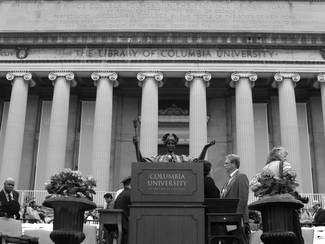
\includegraphics[width=325pt]{columbia.png}
The 259th Commencement of Columbia University in the City of New York \\
22 May 2013 \\
{\tt kula.tproa.net/photos/2013/2013-columbia-graduation/}
\end{center}

\newpage

\thispagestyle{empty}
\vspace*{12cm}
\begin{sideways}
\Large{St. Joshua Norton Press}
\end{sideways}
\begin{sideways}
\Large{PO Box 250138}
\end{sideways}
\begin{sideways}
\Large{New York NY 10025}
\end{sideways}


\end{document}


